\section*{Introduction}

\begin{frame}{Introduction}
\begin{columns}[c]
    \begin{column}{0.05\textwidth}
    \end{column}\begin{column}{0.3\textwidth}
        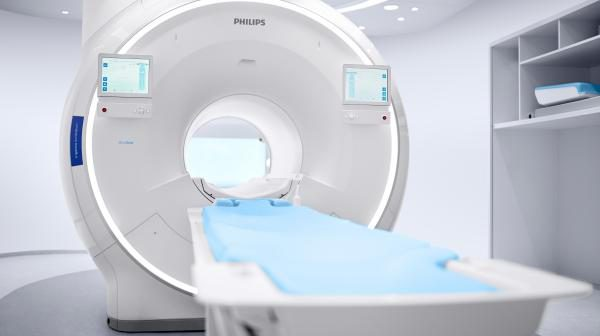
\includegraphics[width=\textwidth]{images/01_introduction/mri.jpg}
    \end{column}\begin{column}{0.3\textwidth}
        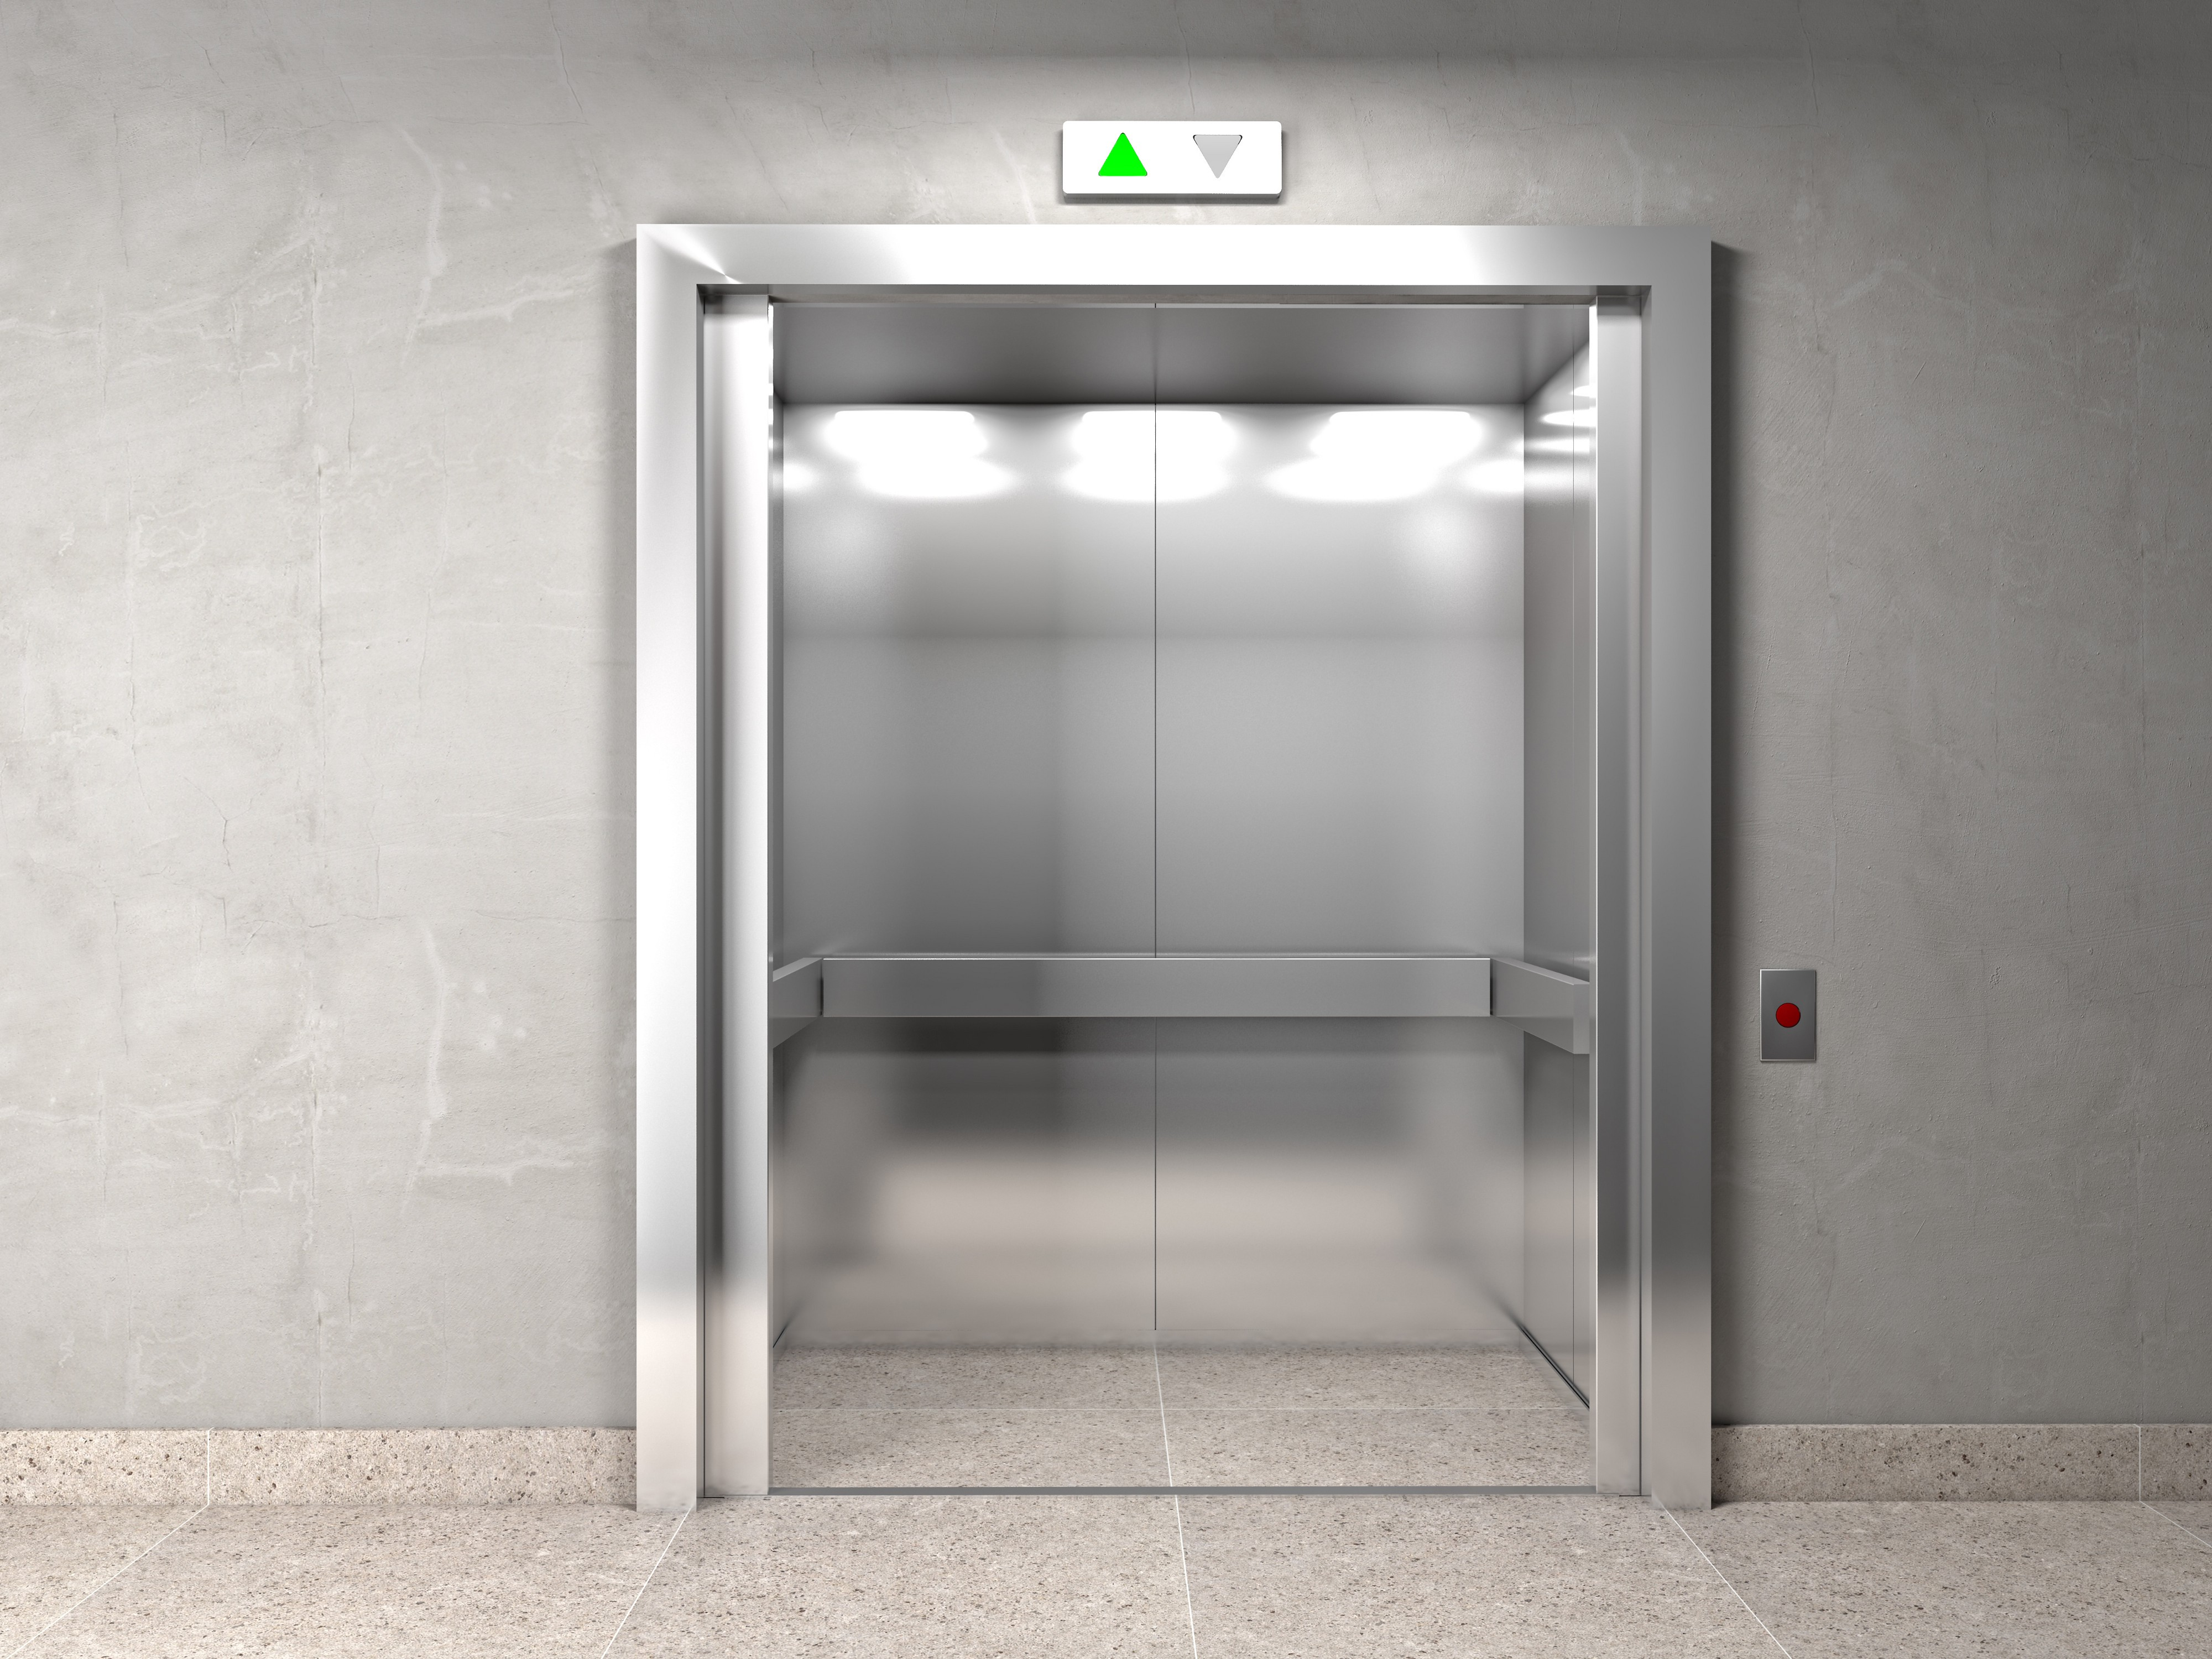
\includegraphics[width=\textwidth]{images/01_introduction/elevator.jpg}
    \end{column}\begin{column}{0.3\textwidth}
        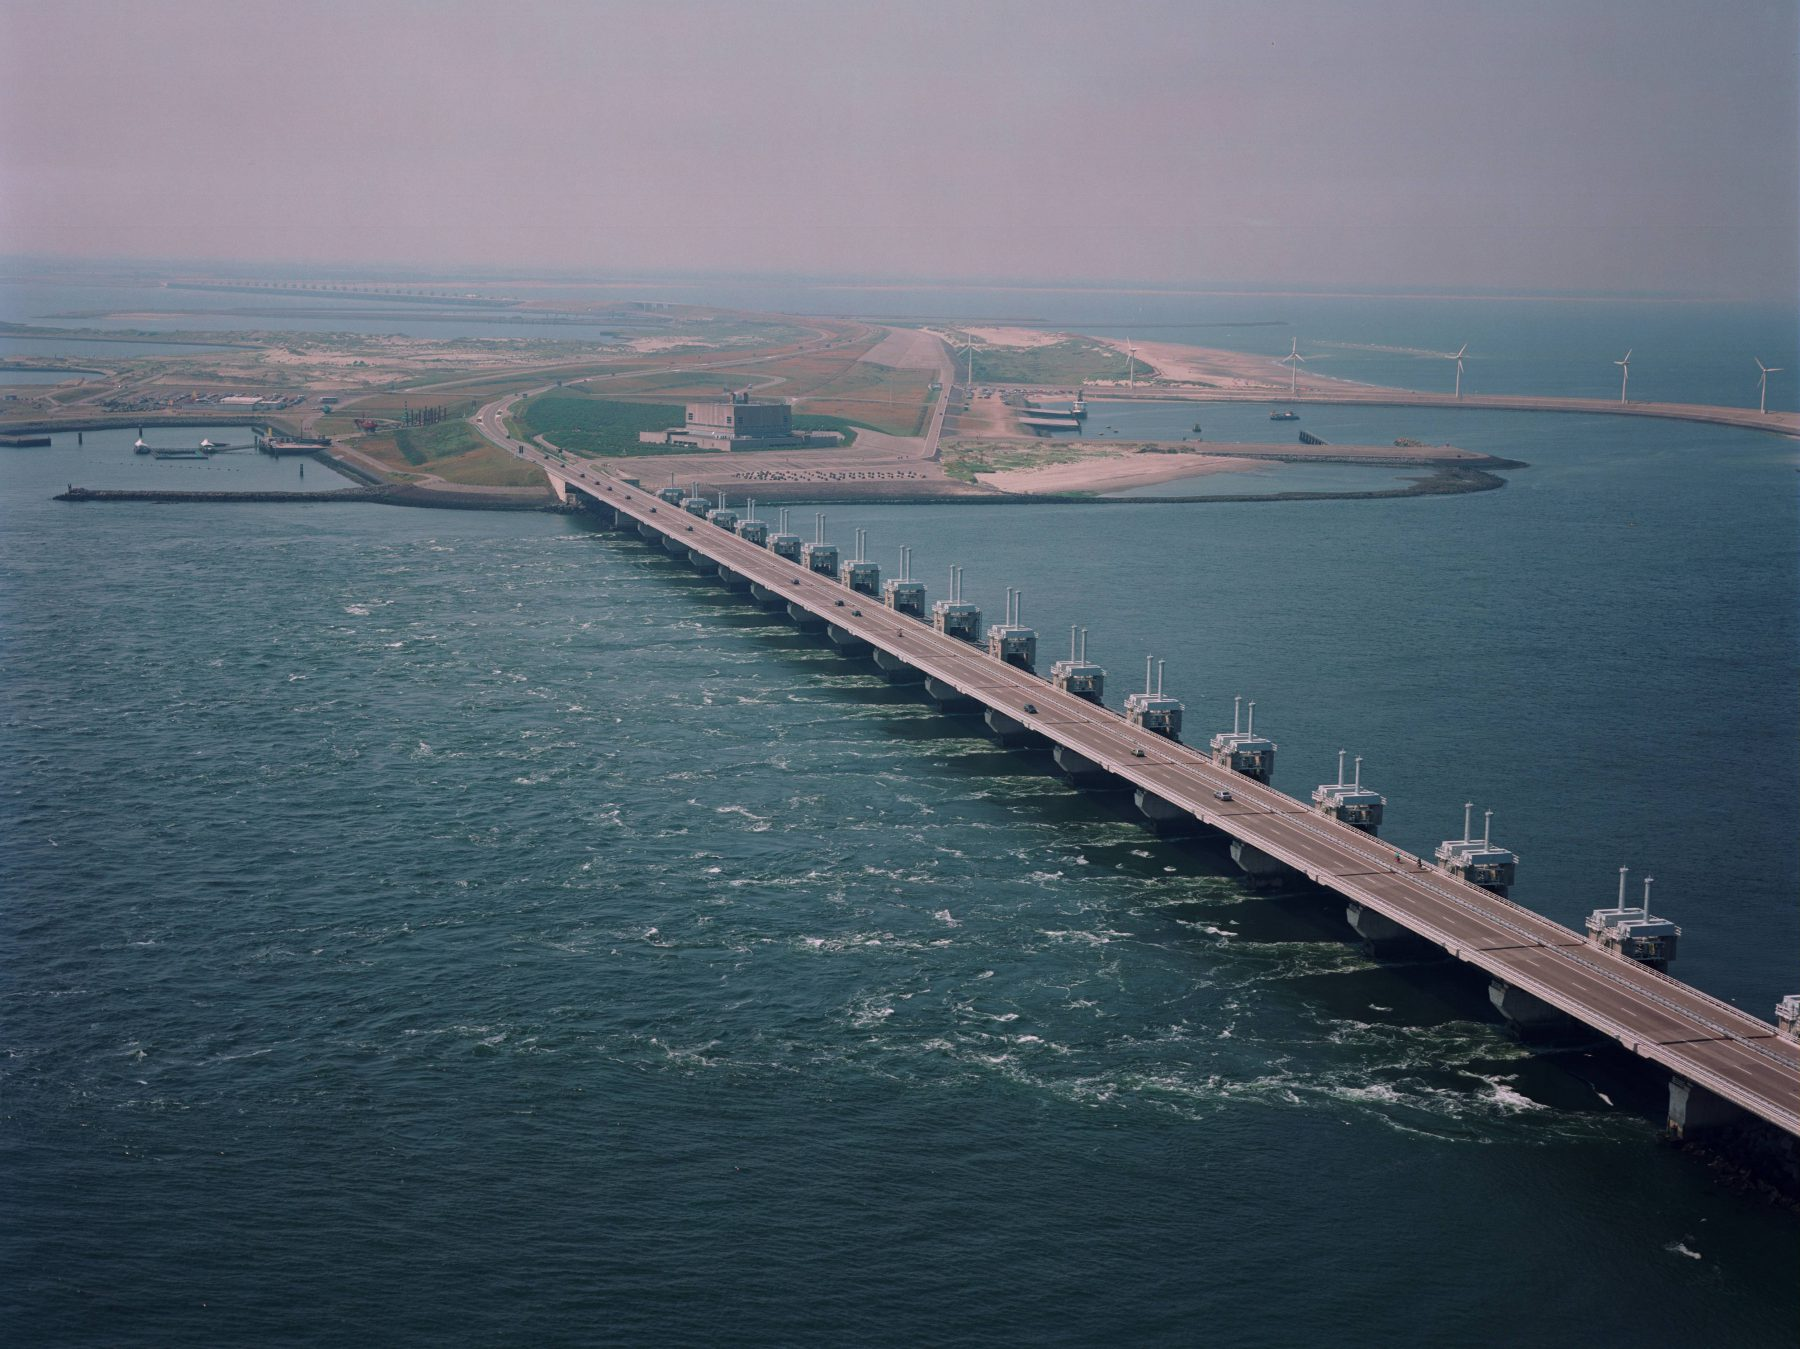
\includegraphics[width=\textwidth]{images/01_introduction/oosterscheldekering.jpg}
    \end{column}
\end{columns} 
\end{frame}

\note{
	\begin{itemize}
	    \item What have these 3 images in common?
	    \item They all make use of software systems that are crucial to be error free
	    \item How to ensure that software is error-free? Through software verification.
	\end{itemize}
}

\begin{frame}{Software verification through models}
    \centering
    \begin{tikzpicture} 
    \path
    (-3,1.5) node[inner sep=0pt](model) {% To use this figure in your LaTeX document
% import the package groove/resources/groove2tikz.sty
%
\begin{tikzpicture}[scale=0.6, every node/.style={scale=0.3}, name prefix=type-]
\node[type_node] (n0) at (0.560, -0.290) {\ml{\textbf{House}\\name: \textbf{string}}};
\node[type_node] (n1) at (0.600, -1.430) {\ml{\textbf{Room}\\number: \textbf{int}}};
\node[type_node] (n2) at (2.470, -1.435) {\ml{\textbf{Renter}}};
\node[type_node] (n3) at (2.470, -2.175) {\ml{\textit{\textbf{PaymentInterval}}}};
\node[type_node] (n4) at (1.070, -2.785) {\ml{\textbf{PaymentInterval\$MONTH}}};
\node[type_node] (n5) at (3.430, -2.785) {\ml{\textbf{PaymentInterval\$QUARTER}}};
\node[type_node] (n6) at (2.470, -0.375) {\ml{\textit{\textbf{Person}}\\age: \textbf{int}\\name: \textbf{string}}};

\path[subtype_edge](n2.north -| 2.470, -0.375) --  (n6) ;
\path[subtype_edge] (n4)  --  (n3) ;
\path[subtype_edge] (n5)  --  (n3) ;
\path[basic_edge](n2.west |- 0.600, -1.430) -- node[lab] {\ml{rents}} (n1) ;
\path[basic_edge, composite](n0.south -| 0.600, -1.430) -- node[lab] {\ml{rooms}} (n1) ;
\path[basic_edge](n2.south -| 2.470, -2.175) -- node[lab] {\ml{payment\_interval}} (n3) ;
\path[basic_edge](n1.east |- 2.470, -1.435) -- node[lab] {\ml{renter}} (n2) ;
\end{tikzpicture}
}
    (-3,-1.5) node[inner sep=0pt](checklist) {
\includegraphics[width=1.5cm]{images/01_introduction/checklist.pdf}}
    (0,0) node[inner sep=0pt](app) {
\includegraphics[width=2cm]{images/01_introduction/application.pdf}}
    (3,1.5) node[inner sep=0pt](correct) {\fontsize{40}{48} \selectfont \textcolor{ForestGreen}{\checkmark}}
    (3,-1.5) node[inner sep=0pt](incorrect) {\fontsize{40}{48} \selectfont \textcolor{red}{\ding{53}}};
    
    \path[]		
    (model) [-{Latex[width=10]}, black] edge node[above] {} (app)
    (checklist) [-{Latex[width=10]}, black] edge node[above] {} (app)
    (app) [-{Latex[width=10]}, black] edge node[above] {} (correct)
    (app) [-{Latex[width=10]}, black] edge node[above] {} (incorrect)
    ;
    \end{tikzpicture}
\end{frame}

\note{
    Explain the automated verification using a tool
	\begin{itemize}
	    \item Software model and the requirements that should be checked are given to verification software.
	    \item Verification software checks these requirements on the model.
	    \item It produces a result.
	\end{itemize}
	I will focus on obtaining the models that can be used for verification.
}

\begin{frame}{Software verification through models}
    \centering
    \begin{tikzpicture} 
    \path
    (-8,1.5) node[inner sep=0pt](fstmodel) {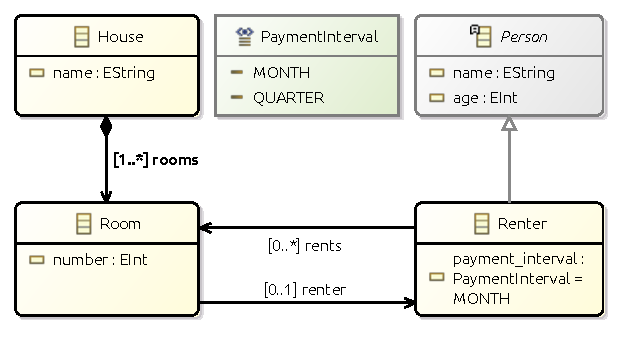
\includegraphics[width=3cm]{images/01_introduction/fstmodel.pdf}}
    (-3,1.5) node[inner sep=0pt](model) {% To use this figure in your LaTeX document
% import the package groove/resources/groove2tikz.sty
%
\begin{tikzpicture}[scale=0.6, every node/.style={scale=0.3}, name prefix=type-]
\node[type_node] (n0) at (0.560, -0.290) {\ml{\textbf{House}\\name: \textbf{string}}};
\node[type_node] (n1) at (0.600, -1.430) {\ml{\textbf{Room}\\number: \textbf{int}}};
\node[type_node] (n2) at (2.470, -1.435) {\ml{\textbf{Renter}}};
\node[type_node] (n3) at (2.470, -2.175) {\ml{\textit{\textbf{PaymentInterval}}}};
\node[type_node] (n4) at (1.070, -2.785) {\ml{\textbf{PaymentInterval\$MONTH}}};
\node[type_node] (n5) at (3.430, -2.785) {\ml{\textbf{PaymentInterval\$QUARTER}}};
\node[type_node] (n6) at (2.470, -0.375) {\ml{\textit{\textbf{Person}}\\age: \textbf{int}\\name: \textbf{string}}};

\path[subtype_edge](n2.north -| 2.470, -0.375) --  (n6) ;
\path[subtype_edge] (n4)  --  (n3) ;
\path[subtype_edge] (n5)  --  (n3) ;
\path[basic_edge](n2.west |- 0.600, -1.430) -- node[lab] {\ml{rents}} (n1) ;
\path[basic_edge, composite](n0.south -| 0.600, -1.430) -- node[lab] {\ml{rooms}} (n1) ;
\path[basic_edge](n2.south -| 2.470, -2.175) -- node[lab] {\ml{payment\_interval}} (n3) ;
\path[basic_edge](n1.east |- 2.470, -1.435) -- node[lab] {\ml{renter}} (n2) ;
\end{tikzpicture}
}
    (-3,-1.5) node[inner sep=0pt](checklist) {
\includegraphics[width=1.5cm]{images/01_introduction/checklist.pdf}}
    (0,0) node[inner sep=0pt](app) {
\includegraphics[width=2cm]{images/01_introduction/application.pdf}}
    (3,1.5) node[inner sep=0pt](correct) {\fontsize{40}{48} \selectfont \textcolor{ForestGreen}{\checkmark}}
    (3,-1.5) node[inner sep=0pt](incorrect) {\fontsize{40}{48} \selectfont \textcolor{red}{\ding{53}}};
    
    \path[]
    (fstmodel) [-{Latex[width=10]}, black] edge node[above] {Transform} (model)
    (model) [-{Latex[width=10]}, black] edge node[above] {} (app)
    (checklist) [-{Latex[width=10]}, black] edge node[above] {} (app)
    (app) [-{Latex[width=10]}, black] edge node[above] {} (correct)
    (app) [-{Latex[width=10]}, black] edge node[above] {} (incorrect)
    ;
    \end{tikzpicture}
\end{frame}

\begin{frame}{Model transformations}
    \begin{itemize}
        \item Concept from Model-driven engineering (MDE)
        \item Use a systematic approach to transform models within/between modelling languages
        \item For use in software verification, a formal foundation is required.
    \end{itemize}
\end{frame}

\note{
	\begin{itemize}
	    \item Explain that transforming models is a concept borrowed from MDE.
	    \item Explain that for verification, we want the model transformations to be proven correct, however, in most implementations this is not the case.
	\end{itemize}
}

\begin{frame}{Scope}
    \begin{itemize}
        \item Model transformations between
        \begin{itemize}
            \item EMF/Ecore
            \item GROOVE graphs
        \end{itemize}
        \item Only syntactical correctness is proven
    \end{itemize}
\end{frame}

\note{
	\begin{itemize}
	    \item Explain that my thesis focuses on solely 2 languages.
	    \item Explain that only syntactical correctness is considered within this work. Sematics are left for future work.
	\end{itemize}
}

\begin{frame}{Research questions}
    What is a suitable formalisation for composable model transformations between Ecore and GROOVE that gives rise to correct model transformations between Ecore and GROOVE?
    \pause
    \begin{itemize}
        \item What is a suitable formalisation of Ecore models and what Ecore models are valid within this formalisation? 
        \item What is a suitable formalisation of GROOVE grammars and what GROOVE grammars are valid within this formalisation? 
        \pause
        \item What is a suitable formalisation for the model transformations between Ecore and GROOVE?
        \item What model transformations are correct within the formalisation?
        \pause
        \item How can correct model transformations between Ecore and GROOVE be composed?
    \end{itemize}
\end{frame}

\note{
	\begin{itemize}
	    \item Explain the main research question. We already discussed the ingredients of the problem, so we can use that.
	    \begin{itemize}
	        \item The first two subquestions discuss the formal descriptions of EMF/Ecore and GROOVE.
	        \item The third subquestion discusses the formal description of the model transformations.
	        \item The fourth question discusses the correctness properties.
	        \item The last question is about composability, see below.
	    \end{itemize}
	    \item Leave composability on a cliffhanger. This is the only detail that was not discussed yet. In order to explain this in detail, we should first see why composability is a nice property to have, which is discussed as part of the next section.
	\end{itemize}
}

\begin{frame}{Validation}
    \begin{itemize}
        \item All proofs are checked using Isabelle, a theorem prover.
        \item Example applications show the feasibility and existance of correct model transformations.
    \end{itemize}
\end{frame}

\note{
	\begin{itemize}
	    \item The work contains a lot of mathematical formalisations and proofs, validating these is done through Isabelle, a proof assistant.
	    \item Explain that a formalisation is useless if no correct model transformations exist. An application of the proven theory shows that this is not the case.
	\end{itemize}
}

\begin{frame}{Contribution}
    Existing work on the formalisation of model transformations exists. Most important work is in the area of Triple Graph Grammars.\\
    \pause
    \vspace{0.5cm}
    What is the contribution of this thesis?
    \begin{itemize}
        \item Different approach, no conversion to graphs
        \item First formalisation of transformations between Ecore \& GROOVE specifically
    \end{itemize}
\end{frame}

\note{
	\begin{itemize}
	    \item Explain that there is earlier work on the formalisation of model transformations. Most important work is in the area of TGGs, which use graph formalisations for the modelling languages.
	    \item Explain the contribution of this work, which does not use triple graph grammars, which is an entirely different approach.
	    \item Moreover, this work focuses on Ecore/GROOVE transformations specifically, which gives rise to an formalisation that is concrete considering existing work.
	\end{itemize}
}

\begin{frame}{Contents}
\tableofcontents
\end{frame}